\capitulo{3}{Conceptos teóricos}

El proyecto tiene una relación directa con la minería de datos y los conceptos que lo rodean. 

\section{Aprendizaje automático (\textit{machine learning})}\label{sec:machine-learning}
En~\cite{sanchez_2020} se define el aprendizaje automático (\textit{machine learning}) como una rama dentro del campo de la Inteligencia Artificial que proporciona a los sistemas la capacidad de aprender y mejorar de manera automática, a partir de la experiencia. Estos sistemas transforman los datos en información, y con esta información pueden tomar decisiones. Este tipo de modelos se crean a base del uso masivo de datos. Cuando se dispone de los datos suficientes para entrenar un modelo comienza el proceso de aprendizaje. El objetivo de este aprendizaje es descubrir patrones ocultos en los datos. En muchas ocasiones el resultado del aprendizaje, el modelo, es una función que dadas unos datos de entrada clasifica o predice correctamente una salida. Como se puede ver en la Figura~\ref{fig:Machine-learning-overview} el aprendizaje automático, \textit{machine learning}, posee diferentes aproximaciones, siendo la interfaz diferenciadora entre ellas la forma de uso de las instancias.
\imagenFlotante{../img/memoria/Machine-learning-overview.pdf}{\textit{Machine learning overview}~\cite{technovert_2020}.}{Machine-learning-overview}

\subsection{Aprendizaje supervisado}\label{subsec:Aprendizaje-Supervisado}
El aprendizaje automático puede ser resumido como <<aprender de ejemplos>>. Al programa se le proporcionan dos conjuntos de datos, uno de entrenamiento y otro de validación~\cite{learned2014introduction}. El objetivo es simple, debe de <<aprender>> en función del conjunto de datos etiquetado proporcionado como entrenamiento para posteriormente identificar las correspondientes etiqueta/s de cada instancia del conjunto de validación con la mayor precisión posible. 

Dependiendo del tipo de etiqueta, en el aprendizaje supervisado hay dos modelos~\cite{supervised_learning_mathworks_inc}.
\begin{enumerate}
	\item \textbf{Modelos de clasificación.} Producen como salida una etiqueta discreta, \textit{i.e.} una etiqueta dentro de un conjunto finito de etiquetas, habitualmente suelen ser o binarias $[0,1]$, $[sí,no]$... o multi-etiqueta, donde por ejemplo los valores pueden variar $[0...n]$, \textit{i.e.} no tienen que ser estrictamente numéricas, pudiendo ser categóricas como por ejemplo $\lbrace coche, moto, barco\rbrace$. En los modelos de clasificación multi-etiqueta es habitual que el clasificador trabaje con selección de varias etiquetas para la misma muestra, no estando restringido a una única~\cite{tsoumakas2007multi}.

Entre los algoritmos de clasificación más frecuentes encontramos:
	\begin{itemize}
	\item Regresión logística.
	\item \textit{Support Vector Machine, SVM}.
	\item Redes neuronales.
	\item Clasificador Naïve Bayes.
	\item Árbol de decisión.
	\item Análisis discriminante.
	\item \textit{K} vecinos más cercanos, \textit{KNN}.
	\item Clasificación con ensembles.
	\end{itemize}
	\item \textbf{Modelos de regresión.} Producen como salida un valor real, numérico. Suelen ser soluciones continuas. De igual manera si se quieren obtener varios resultados de una muestra, se denomina multi-\textit{output}~\cite{borchani2015survey}.
	
	Entre los algoritmos de regresión más frecuentes encontramos:
	\begin{itemize}
	\item Regresión lineal.
	\item Regresión no lineal.
	\item Modelo lineal generalizado.
	\item Árbol de decisión.
	\item Redes neuronales.
	\item Regresión con procesos gaussianos.
	\item Regresión con \textit{support vector machines}.
	\item Regresión con ensembles.
	\end{itemize}
	
\end{enumerate}

\subsection{Aprendizaje no supervisado}\label{subsec:Aprendizaje-No-Supervisado}
En la Sección~\ref{subsec:Aprendizaje-Supervisado} se comenta que, los modelos para que <<aprendan>> los patrones que se encuentran en los conjuntos de datos, necesitan tener un conjunto de datos etiquetado correctamente para extraer la información de ese conjunto. Pero en los problemas del mundo real no siempre se tienen infinidad de datos disponibles etiquetados correctamente, o simplemente es un proceso muy laborioso y costoso económicamente.

Para solventar este problema se cuenta con el aprendizaje no supervisado~\cite{bengio2012unsupervised}, mediante esta técnica no es necesario proporcionar al modelo datos etiquetados. Por definición, el algoritmo encargado de entrenar el modelo  <<aprenderá>> los datos sin conocimiento previo. Para ello el modelo se basará en los datos que tiene disponibles y en la codificación del algoritmo para descubrir los patrones que se encuentren en los datos.

Debido a la forma de trabajar del aprendizaje no supervisado, desde el primer momento en el que el algoritmo tiene los datos comienza a reportar salidas, describiendo la información y categorizando lo que encuentra en los mismos.

Principalmente existen dos técnicas de aprendizaje no supervisado.
\begin{enumerate}
	\item \textbf{\textit{Clustering}}~\cite{unsupervised_learning_clustering}. Proceso por el cual se dividen los datos no clasificados en grupos aparentemente similares. Cuando se identifican datos con algún parecido entre sí, son agrupados. Permite clasificar e identificar atributos únicos de los datos con los que clasificarlos. 
	
	Un proceso habitual de agrupamiento es el uso de \textit{K-means}, $K\in\mathbb{R}$, donde se indica en $K$ cuántos \textit{clusters} o grupos se han de identificar en los datos.
	
	Con los datos agrupados el proceso de análisis de éstos puede comenzar. En ocasiones si el número de grupos detectados es muy alto, se pueden encontrar grupos o \textit{clusters} irrelevantes, permitiendo a los científicos de datos eliminar esos datos que los forman, reduciendo la dimensionalidad~\cite{boutsidis2014randomized}.
	
	\item \textbf{Reducción de la dimensionalidad}~\cite{li2002unsupervised}. El aprendizaje se basa en instancias/ejemplos y éstos a su vez están formados por atributos o características, lo cual permite su clasificación, valga la redundancia. Cuando los conjuntos de datos poseen múltiples características, más difícil resulta su clasificación. Es por ello que resulta útil identificar aquellos atributos que están fuertemente interrelacinados entre sí para eliminar todos menos un atributo, reduciendo la dimensionalidad~\cite{li2002unsupervised}.
\end{enumerate}

\subsection{Aprendizaje semi-supervisado}\label{subsec:Aprendizaje-Semi-Supervisado}
Según~\cite{zhou2014semi} \textit{Semi-Supervised Learning} se define como una forma de entrenamiento de modelos el cual usa tanto datos etiquetados como no etiquetados, \textit{i.e.} si no sería un aprendizaje supervisado, o no supervisado. 

El uso de aprendizaje semi-supervisado se caracteriza por ser menos costoso que el supervisado, ya que este último necesita que todo el conjunto de datos que va a utilizar para aprender esté etiquetado, y ese proceso es normalmente costoso (en tiempo y en recursos). Luego, obtiene mejores resultados en menor tiempo que el aprendizaje no supervisado. 
Conseguir datos sin etiquetar es una tarea muy sencilla, mientras que conseguir conjuntos de datos etiquetados es un proceso complejo y actualmente no hay <<de todo>>.

Para que el aprendizaje sea fructuoso requiere que las instancias se encuentren inter-relacionadas entre sí por alguna de sus características~\cite{javatpoint_semisupervised} indica las siguientes suposiciones que se dan en el aprendizaje semi-supervisado.
\begin{enumerate}
	\item \textbf{Continuity} o continuidad. Se asume que los objetos cercanos entre sí se encontrarán en el mismo \textit{cluster} o grupo de etiquetas. 
	\item \textbf{\textit{Clustering}} o agrupamiento. Las instancias son divididas en diferentes grupos discretos, compartiendo todos los elementos de un \textit{cluster} la misma etiqueta.
	\item \textbf{\textit{Manifold}} o variedad. Se emplea el uso de distancias y funciones de densidad de forma que las instancias se encuentran en colectores con menos dimensiones que el espacio de entrada.
\end{enumerate}

Dentro de las \textit{best practices} en \textit{semi-supervised learning} se encuentran el uso de diferentes modelos de redes neuronales para el entrenamiento~\cite{thekumparampil2018attention}.


\section{Algoritmos de aprendizaje semi-sepervisado}\label{sec_alg:semi-supervised}
A continuación se van a presentar los algoritmos implementados en este trabajo dentro del aprendizaje semi-supervisado.

\subsection{\textit{Self-training}}
Los métodos de auto-etiquetado (\textit{self-training}), son uno de los métodos más sencillos de pseudo-etiquetado que existen~\cite{triguero2015self}. Consisten en un único clasificador el cual utiliza aprendizaje supervisado, el clasificador es entrenado con datos etiquetados conocidos al comienzo del entrenamiento y por los que se van conociendo a medida que pasan las iteraciones. Es decir, el clasificador inicialmente es entrenado con aquellos datos para los que se posea una etiqueta, y en sucesivas iteraciones se le reentrenará con el nuevo conjunto de datos etiquetado, que es el resultante de añadir a los datos etiquetados previos, aquellas predicciones con un elevado \textit{condifence level}~\cite{jesper2020survey}.

Yarowsky~\cite{yarowsky1995unsupervised} en 1995 propuso la primera versión de \textit{Self-training}, desde entonces numerosas aproximaciones han sido realizadas, modificando la utilización del conjunto de datos etiquetado, los nuevos datos, etcétera. El diseño que se le puede dar y los campos de aplicación del mismo son muy variados.

El procedimiento de selección de qué datos son pseudo-etiquetados es de vital importancia, puesto que determinará qué datos acaban en el conjunto de datos etiquetado de sucesivas iteraciones. Siendo este un proceso iterativo y no incremental, ya que la probabilidad de etiquetado de los datos es re-calculada en cada iteración. De no serlo sería una apoximación a \textit{expectation-maximization}~\cite{dempster1977maximum}.

\subsection{\textit{Co-Training}}
Blum~\cite{blum1998combining} en 1998 propuso el \textit{Co-Training} para conjuntos de datos compuestos por datos separables en dos vistas. Bajo la presunción de que con unos pocos datos etiquetados y diferentes clases que aportan información, se pueden entrenar dos algoritmos de aprendizaje por separado para posteriormente añadir al conjunto de datos etiquetados aquellas predicciones con un mayor intervalo de confianza (\textit{confidence level}).

Las dos características del problema mencionadas anteriormente, disponibilidad de datos etiquetados y no etiquetados, y la disponibilidad de dos <<tipos>> diferentes de conocimiento sobre los ejemplo; aproximan a la siguiente estrategia de aprendizaje. Se desea encontrar los predictores débiles basados en cada tipo de información utilizando un pequeño conjunto inicial de instancias etiquetadas, seguidamente, utilizando los datos no etiquetados se intenta hacer un \textit{bootstrap} a partir de esos <<malos>> predictores. Este tipo de \textit{bootstrapping} es el denominado \textit{Co-Training}, y posee una estrecha relación con el \textit{bootstrapping} a partir de datos incompletos en el marco de la maximización de expectativas~\cite{ghahramani1994supervised, ratsaby1995learning}.

\begin{algorithm}[H]
	\KwIn{Conjunto de entrenamiento $L \lbrace\left(x_i, y_i\right)\rbrace_{i=1}^l$ y $U \lbrace x_j \rbrace_{j=l+1}^{l+u}$ de datos etiquetados y no etiquetados, respectivamente}
	\KwIn{$p$, $n$, $k$, $u$, datos positivos a seleccionar, los negativos, iteraciones, tamaño \textit{pool} inicial}
  	\BlankLine
  	$U' \leftarrow U[u]$\tcc*[f]{$u$ instancias aleatorias de $U$}\\
  	\For{k}{
		Usar $L$ para entrenar un clasificador $h_1$ utilizando $x$\\
		Usar $L$ para entrenar un clasificador $h_2$ utilizando $y$\\
		$h_1$ clasifica $U'$\\
		$h_2$ clasifica $U'$\\
		Seleccionar las $p$ y $n$ instancias con mayor intervalo de confianza de cada clasificador\\
		Añadirlas a $L$ y eliminarlas de $U'$\\
		Elegir aleatoriamente $2p+2n$ instancias de $U$ y añadirlas a $U'$\\
	}
	\caption{\textit{Co-Training}}\label{alg:Co-Training}
\end{algorithm}

\subsection{\textit{Tri-Training}}
Zhou~\cite{zhou2005tri} en 2005 propuso una modificación sobre el algoritmo de \textit{Co-Training} de Blum~\cite{blum1998combining}. Dasgupta~\textit{et al.}~\cite{dasgupta2002pac} demostraron que cuando los requerimientos del conjunto de datos se cumplían, se podían producir un menor número de errores de generalización al maximizar la clasificación de los prototipos sin etiquetar, aunque no es aplicable a cualquier conjunto de datos.

El \textit{Tri-Training} se define como una nueva aproximación de \textit{Co-Training}. \textit{Tri-Training} no necesita varias <<vistas significativas>> de los datos, tampoco requiere el empleo de múltiples algoritmos de aprendizaje supervisado cuyas hipótesis dividen el espacio de instancias en un conjunto de clases de equivalencia. El \textit{Tri-Training} por tanto emplea tres clasificadores, a diferencia de los dos utilizados anteriormente, esta opción resuelve la dificultad de determinar cómo etiquetar las instancias no etiquetadas y generar la hipótesis final, lo que mejora enormemente la eficiencia del algoritmo. Junto con la capacidad de generalización resultante de la combinación de los tres clasificadores.

\begin{algorithm}[H]
	\KwIn{Conjunto de entrenamiento $L$ y $U$ de datos etiquetados y no etiquetados, respectivamente}
	\KwIn{\textit{Learn}\tcc*[f]{algoritmo de aprendizaje}}
  	\BlankLine
	\For{$i \in \lbrace 1\dots 3 \rbrace$}{
		$S_i \leftarrow BootstrapSample(L)$\\
		$h_i \leftarrow Learn(S_i)$\\
		$e'_i \leftarrow 0,5$\\
		$l'_i \leftarrow 0$
	}
	\Repeat{ningún $h_i \left(i \in \lbrace 1\dots3\rbrace\right)$ cambie}{
		\For{$i \in \lbrace 1\dots 3\rbrace$}{
			$L_i \leftarrow \emptyset$\\
			$update_i \leftarrow$ \textbf{False}\\
			$e_i \leftarrow MeasureError\left(h_j \& h_k \right)$ $\left(j\text{,}k \not= i \right)$\\
			\If{$e_i < e'_i$}{
				\ForAll{$x \in U$}{
					\If{$h_j\left( x\right) = h_k \left(x\right)$ $\left(j\text{,}k \not= i \right)$}{
						$L_i \leftarrow L_i \cup \lbrace \left( x\text{,} h_j\left(x\right)\right)\rbrace$
					}
				}
				\If{$l'_i = 0$}{
					$l'_i \leftarrow \left\lfloor \frac{e_i}{e'_i-e_i} + 1 \right\rfloor$
				}
				\uIf{$l'_i < \left| L_i \right|$}{
					$update_i \leftarrow$ \textbf{True}
				}
				\ElseIf{$l'_i > \frac{e_i}{e'_i-e_i}$}{
					$L_i \leftarrow Subsample\left( L_i\text{,} \left\lceil \frac{e'_il'_i}{e_i} - 1 \right\rceil \right)$\\
					$update_i \leftarrow$ \textbf{True}
				}
			}
		}
		\For{$i \in \lbrace 1 \dots 3 \rbrace$}{
			\If{$update_i =$ \textbf{True}}{
				$h_i \leftarrow Learn\left( L \cup L_i\right)$\\
				$e'_i \leftarrow e_i$\\
				$l'_i \leftarrow \left|L_i\right|$\\
			}
		}
	}
  	
	\caption{\textit{Tri-Training}}\label{alg:Tri-Training}
\end{algorithm}

Los tres clasificadores, $h_1\text{, } h_2 \text{ y } h_3$, son entrenados inicialmente con todo el conjunto de datos etiquetado. Seguidamente, a cualquier instancia no etiquetada, se la podrá asignar una etiqueta siempre y cuando hay al menos dos clasificadores de acuerdo con la asignación, \textit{i.e.} $label(x) = h_i(x) =  h_j(x)$, ver~ algoritmo~\ref{alg:Tri-Training}. Puede darse el caso de que dos clasificadores acierten en la predicción y la etiqueta sea considerada correcta, pero para el tercer clasificador sea ruido, incluso en el peor caso, el aumento del ruido en el proceso de clasificación puede mitigarse si el número de instancias recién etiquetadas es significativo (bajo condiciones específicas)~\cite{zhou2005tri}.

Debido a que \textit{Tri-Training} no asume la existencia de clases <<redundantes>>, se necesita un cierto grado de diversidad en los clasificadores. Esta diversidad es alcanzada mediante la manipulación del conjunto de datos etiquetado. Los clasificadores iniciales son entrenados con los datos generados mediante \textit{bootstrap}\footnote{En el campo de la estadística, se define como un método el cual consiste en la extracción de datos de muestra repetidamente con reemplazo de un conjunto de datos, con el fin de estimar un parámetro de la población.} del conjunto de datos etiquetados original. Estos clasificadores son depurados en el proceso iterativo del algoritmo, produciendo la hipótesis final mediante mayoría simple.

Dado que \textit{Tri-Training} no impone ninguna restricción al algoritmo de aprendizaje supervisado ni emplea un proceso de validación cruzada que requiera mucho tiempo de cómputo, tanto su aplicabilidad como su eficiencia demuestran ser mejores que otras versiones de \textit{Co-Training}.

\subsection{\textit{Democratic Co-Training}}
Zhou~\cite{zhou2004democratic} en 2004 presentó el algoritmo \textit{Democratic Co-Learning}. El algoritmo a diferencia de sus <<homónimos>>, trabaja con múltiples algoritmos de aprendizaje supervisado, en lugar de múltiples clases significativas, permitiendo que se etiqueten nuevas instancias entre ellos. Debido a que diferentes algoritmos de aprendizaje poseen diferentes sesgos, seleccionar la clase más votada por la mayoría produce mejores predicciones.

El algoritmo es por tanto enfocado para el uso en casos donde no existen dos conjuntos de atributos independientes y redundantes, su pseudocódigo se encuentra disponible en los algoritmos~\ref{alg:Democratic-Co}~y~\ref{alg:Democratic-Co-2}.

Es por ello que \textit{Democratic Co-Learning} utiliza un conjunto de datos etiquetados, \textit{L}, uno de no etiquetados, \textit{U}, y $A_1,\dots ,A_n$ para $n \geq 3$, siendo $n$ los algoritmos de aprendizaje supervisado, ver Algoritmo~\ref{alg:Democratic-Co}. El algoritmo comienza entrenando los $n$ clasificadores sobre el conjunto de datos etiquetado $L$; y para cada instancia $x$ del conjunto de no etiquetados $U$, cada clasificador predice una etiqueta $c_i \in \mathcal{C} = \lbrace c_1, c_2, \dots , c_r\rbrace$. Siendo $c_k$ la predicción mayoritaria. Posteriormente los $n$ clasificadores son re-entrenados con los nuevos datos etiquetados (añadidos a los que ya teníamos), este proceso se realiza de manera iterativa hasta que no se seleccionen más datos para realizar el etiquetado. Para la selección final se realizar un voto mayoritario ponderado entre los $n$ clasificadores. 

Una instancia $x$ nunca será etiquetada por la decisión única de un clasificador, a menos que la mayoría de los clasificadores estén de acuerdo. Además se requiere que la suma de los valores medios de confianza de los clasificadores del grupo mayoritario sea mayor, que la suma de los valores medios de confianza de los clasificadores de los grupos minoritarios, siendo la confianza media de un clasificador $ (l + h)/2
$ para $l$ y $h$ definidas por el intervalo de confianza del 95\% $\left[l,h\right]$.

Finalizando con la combinación de todas las hipótesis generadas para retornar la hipótesis final. Para realizar el cálculo utiliza un sistema de votación mayoritaria de entre las posibles clases, para hilar un poco más fino, se considera también para cada clasificador su valor de confianza de la predicción. 

\begin{algorithm}[H]
	\KwIn{Conjunto de entrenamiento $L$ y $U$ de datos etiquetados y no etiquetados, respectivamente}
	\KwIn{$A_1,\dots , A_n$ los $n$ algoritmos de aprendizaje supervisado}
  	\BlankLine
	\For{$i = i,\dots , n$}{
		$L_i \leftarrow L$\\
		$e_i \leftarrow 0$ 
	}
	\Repeat{Ningún $L_1, \dots , L_n$ cambie}{
		\For{$i = 1,\dots , n$}{
			Calcular las hip $H_i$ con los datos $L_i$ para cada clasificador $A_i$
		}
		\ForAll{$x \in U$}{
			\For(Posibles etiquetas){$j = 1, \dots, r$}{
				$c_j \leftarrow \left|\lbrace H_i | H_i\left(x\right) = j \rbrace\right|$
			}
			$k \leftarrow arg max_j \lbrace c_j\rbrace$
		}
		\For($x$ propuestos para etiquetar){$i = 1, \dots ,  n$}{
			Utilizar $L$ para calcular el int. de conf. 95\% $\left[l_i, h_i\right]$ para $H_i$\\
			$w_i \leftarrow \left(l_i + h_i \right)/2$\\
			\For{$i = 1, \dots , n$}{
				$L'_i = \emptyset$
			}
			\If{$\sum_{H_j(x) = c_k} w_j > max_{c'_k \not= c_k}\sum_{H_j(x) = c'_k} w_j$}{
				$L'_i \leftarrow L'_i \cup \lbrace\left(x, c_k\right)\rbrace$, $\forall i$ tal que $H_i(x) \not= c_k$
			}
		}
		\tcc{Comprobar si añadir $L'_i$ a $L$ mejora la precisión}
		\For{$i = 1, \dots , n$}{
			$q_i \leftarrow \left| L_i\right| \left(1-2\left(\frac{e_i}{\left|L_i\right|}\right)\right)^2$\tcc*[f]{est. del error}\\
			$e'_i \leftarrow \left(1-\frac{\sum_{i=1}^{d}l_i}{d}\right) \left|L'_i\right|$\tcc*[f]{est. del nuevo error}\\
			$q'_i \leftarrow \left| L_i \cup L'_i \right| \left(1-\frac{2\left(e_i+e'_i\right)}{\left|L_i \cup L'_i\right|}\right)^2$\tcc*[f]{si $L'_i$ es añadida}\\
		}
		\If{$q'_i > q_i$}{
			$e_i \leftarrow e_i + e'_i$
		}
	}  	
	\AlgoSaveLineCount
	\caption{\textit{Democratic Co-Learning}}\label{alg:Democratic-Co}
\end{algorithm}

\begin{algorithm}[H]
	\AlgoRestoreLineCount
	\For{$i=1,\dots , n$}{
		Calcular el int. de conf. 95\% $\left[ l_i, h_i\right]$ para $H_i$ usando $L$\\
		$w_i \leftarrow \left( l_i + h_i\right)/2$
	}
	\ForAll{$x \in \left(L \cup U \right)$}{
		\For{$i = 1, \dots, n$}{
			\If{$H_i(x)$ predice $c_j$ y $w_i > 0.5$}{
				Asociar $H_i$ al grupo $G_j$
			}
		}
		\For{$j = 1, \dots,r$}{
			$\overline{C}_{G_{j}} \leftarrow \frac{\left|G_j\right| + 0.5}{\left|G_j\right| + 1} \times \frac{\sum_{H_i\in G_j}w_i}{\left| G_j\right|}$
		}
	}
	Predicciones $H$ con $G_k$ para $k = argmax_j\left(\overline{C}_{G_{j}}\right)$
	\caption{\textit{Democratic Co-Learning}}\label{alg:Democratic-Co-2}
\end{algorithm}

\subsection{\textit{Self-Training} basado en picos de densidad}
Wu~\cite{wu2018self} en 2018 presentó un \textit{framework} para clasificación utilizando \textit{self-training}. En este caso a diferencia de los métodos estudiados anteriormente, se utilizan técnicas de \textit{clustering} (agrupación) para obtener mejores resultados. Con éste método se descubre la  estructura del espacio de datos, para ello se integra la densidad de los datos en el proceso de \textit{self-training}, de manera que se entrene iterativamente un clasificador. 

El proceso, ver algoritmo~\ref{alg:Wu-DensityPeaks}, por el cuál se consigue este nuevo clasificador <<mejorado>> es el siguiente:
\begin{enumerate}
\item Encontrar los picos de densidad de los datos para aprender la estructura subyacente de todo el espacio de datos de entrenamiento. Y se integra esta estructura en el proceso de entrenamiento iterativo de un clasificador.
\item Se entrena un clasificador con los datos etiquetados. Se clasifican los ejemplos siguientes de los ya etiquetados hasta que no haya más, se predicen y, se añaden y eliminan de los datos etiquetados y no etiquetados, respectivamente.
\item Se repite el paso anterior pero con los puntos anteriores.
\end{enumerate}

\begin{algorithm}[H]
	\KwIn{Conjunto de entrenamiento $L$ y $U$ de datos etiquetados y no etiquetados, respectivamente}
	\KwOut{Clasificador entrenado}
  	\BlankLine
	Calcular $\rho_i$ para cada instancia $x_i \in L \cup U$\\
	Calcular $\delta_i$ para cada instancia $x_i \in L \cup U$\\
	Descubrir la estructura del espacio de datos haciendo que cada $x_i$ <<apunte>> a su 1-NN con mayor $\rho_i$\\
	Entrenar un clasificador $C$ con $L$\\	
	\Repeat{todos los puntos <<siguientes>> de $x_i \in L$ son seleccionados de $U$}{
		Seleccionar un $T$ de $U$ donde cada $x_j$ es un punto <<siguiente>> de los $x_i \in L$
		Etiquetar $x_t \in T$ con $C$\\
		$L \leftarrow L\cup T$\\
		$U \leftarrow U - T$\\
	}
  	Reentrenar $C$ con $L$\\
  	\Repeat{$size:U == 0$}{
		Seleccionar un $T$ de $U$ donde cada $x_j$ es un punto <<anterior>> de los $x_i \in L$
		Etiquetar $x_t \in T$ con $C$\\
		$L \leftarrow L\cup T$\\
		$U \leftarrow U - T$\\
	}
 	Reentrenar $C$ con $L$\\
	\caption{\textit{Self-Training based on Density Peaks}}\label{alg:Wu-DensityPeaks}
\end{algorithm}


\clearpage
\section{Minería de datos}

Según IBM~\cite{IBM-WhatisDataMining}, podemos definir la minería de datos, o descubrimiento de conocimiento
en los datos \textit{Knowledge Discovery in Databases (KDD)}, como el proceso de descubrir patrones y otra
información a partir de grandes conjuntos de datos. 

Las técnicas de minería de datos principales se pueden dividir en función de sus propósitos principales.
\begin{enumerate}
    \item Descripción del conjunto de datos objetivo.
    \item Predicción de resultados mediante el uso de algoritmos de aprendizaje automático.
\end{enumerate}

\subsection{Proceso de minería de datos}
El proceso de minería de datos comprende varios pasos como crear, probar y trabajar con los modelos de minería. Comienza con la recogida de los datos que van a ser tratados, y finaliza con la visualización de la información extraída de éstos. 
Los científicos de datos describen los datos a través de sus observaciones de patrones, asociaciones y correlaciones. A su vez se pueden clasificar y agrupar los datos utilizando métodos de clasificación y regresión.

Uno de los marcos de referencia más importantes en el proceso de minado de datos es CRISP-DM, \textit{Cross Industry Standard Process for Data Mining}. Desarrollado por un consorcio de empresas involucradas en la minería de datos~\cite{Chapman2000CRISPDM1S}.

\begin{figure}
\centering
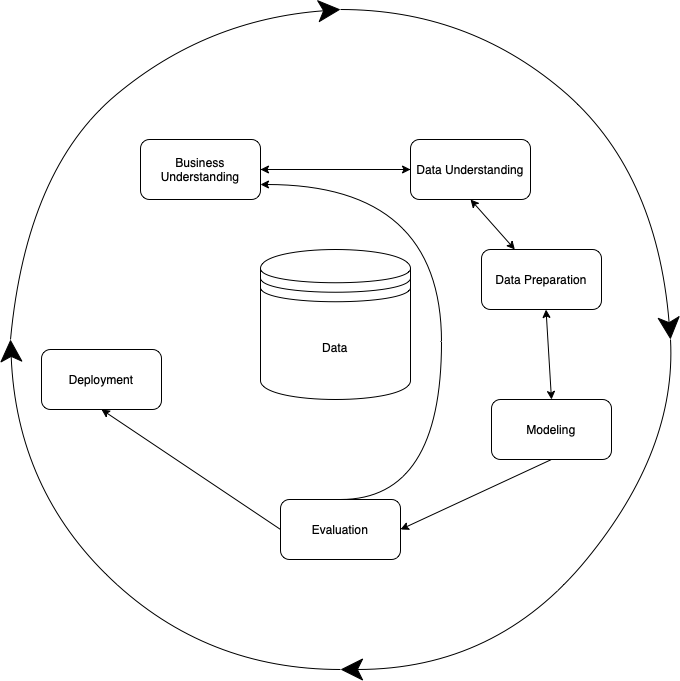
\includegraphics[width=0.7\textwidth]{./img/memoria/CRISP-DM}
\caption{Enfoque CRISP de la minería de datos~\cite{KOTU201517}.}
\label{./img/memoria/CRISP-DM}
\end{figure}

En~\cite{KOTU201517} se divide el proceso de la minería de datos en 5 etapas o pasos principales: establecimiento de los objetivos y comprensión del problema, recopilación y preparación de los datos, desarrollo del modelo, aplicación del modelo y la evaluación de los resultados y despliegue en producción. Ver Figura~\ref{fig:./img/memoria/machine-learning-pipeline}.

\imagen{./img/memoria/machine-learning-pipeline}{\textit{Machine Learning Pipeline}~\cite{mlpipeline2018}.}

\begin{enumerate}
   \item \textbf{Establecer los objetivos y comprensión del problema.}
    La primera etapa puede resultar la más complicada del proceso. Todas las partes interesadas deben de estar presentes y de acuerdo en la definición del problema que se va tratar, esto incluye tanto a los científicos de datos como las terceras partes involucradas o interesadas. 
    Este procedimiento ayuda a la formulación de las preguntas de los datos y los parámetros a utilizar en el proyecto. Si se trata de un proyecto empresarial, se debe hacer un estudio o investigación adicional para comprender el contexto de la empresa.
    \item \textbf{Preparación de los datos.}
    Con el alcance del problema definido ya se puede comenzar a identificar qué conjunto de datos será el más efectivo o representativo con el fin de comenzar a dar respuesta a las preguntas formuladas en el proceso anterior.
    
    Una vez se dispone de todos los datos recogidos comienza el proceso de pre-procesado de los mismos. Este proceso se basa en la limpieza de los datos con el fin de eliminar cualquier posible ruido, entendiéndose por ruido los datos duplicados, los valores perdidos y aquellos atípicos; aquellos que puedan causar problemas a la resolución del problema o generen incertidumbre.
    En determinados conjuntos de datos se puede hacer una reducción de dimensiones. Consiste en la reducción del número de dimensiones que poseen las instancias recogidas, con el fin de eliminar aquellas que no sean realmente representativas o significativas, este proceso reduce la complejidad computacional\footnote{La cuantificación de la dificultad de un problema computacional en términos de recursos informáticos (como el tiempo de cálculo o la cantidad de memoria) necesarios para su solución.} de los cálculos posteriores. Por contrapartida hay que conocer cuáles serán los predictores con mayor relevancia en el problema para garantizar una precisión <<óptima>> del modelo.
    \item \textbf{Desarrollo del modelo.}
    Según~\cite{KOTU201517} el modelo es la representación abstracta de los datos y sus relaciones en un conjunto de datos concreto. Actualmente existen cientos de algoritmos que se pueden utilizar, habitualmente proceden de campos como la ciencia de datos, \textit{machine learning}, o la estadística.
    Se debe tener el conocimiento suficiente para entender cómo funciona el algoritmo para poder configurar correctamente los parámetros que este va a utilizar en base a los datos y el problema de negocio que estamos resolviendo. 
    
En función de cómo los modelos resuelven el problema se pueden clasificar en:
    \begin{enumerate}
        \item Regresión.
        \item Análisis de asociación.
        \item \textit{Clustering.}
        \item Detección de anomalías.
    \end{enumerate}
    
    El modelo debe ser creado con especial cuidado para evitar el \textit{overfitting}, \textit{i.e.} el modelo memoriza el conjunto de entrenamiento y no tendrá un rendimiento correcto una vez desplegado en producción. Se desea que el modelo sea lo más general posible de cara a \textit{aprender} de los datos del conjunto de entrenamiento.

    \item \textbf{Aplicación del modelo.}
	El momento de la aplicación del modelo es cuando de verdad se comprueba si realmente el modelo está listo para pasar al siguiente punto, en otras palabras, si es apto para ser desplegado en producción. 
	Para ello se tienen en cuenta métricas como la calidad del modelo ante el problema, su tiempo de respuesta, etc.
    
	\item \textbf{Evaluación de los resultados y despliegue en producción.}
	Es habitual que los parámetros con los que el modelo fue entrenado con el paso del tiempo dejen de ser los más interesantes, pudiendo ser comprobado el error proporcionado por el modelo con los datos de prueba. Cuando ese error sea excesivo o fuera de un margen dado se deberá de volver a entrenar el modelo, comprobar, y desplegar. 
	De esta forma se puede comprobar como el ciclo de vida del modelo es circular.
\end{enumerate}

El proceso aplicado en la minería de datos proporciona un marco de trabajo mediante el cual se permite extraer información aparentemente no trivial de grandes conjuntos de datos. 
Es un campo de aprendizaje constante, tanto el aplicar los conocimientos del analista para reducir las dimensiones del conjunto de datos, como una vez que se ha entrenado el modelo y puesto en producción, aprender los puntos fuertes de este y el por qué de éstos~\cite{Chapman2000CRISPDM1S}.

\subsection{Técnicas utilizadas en la minería de datos}

A continuación se presentan una serie de técnicas utilizadas en función de la naturaleza de las instancias predictoras, y de la variable de salida. Si la variable o clase de salida es continua o categórica, nos encontramos con modelos de aprendizaje supervisado, mientras que si no existe variable o clase de salida, nos encontramos con modelos de aprendizaje no supervisado~\cite{palmer2011data}.

\begin{enumerate}
	\item \textbf{Reglas de asociación} (además se trata de una técnica de aprendizaje automático). Se basa en el uso de reglas básicas qutilizadas para localizar relaciones entre instancias en conjuntos de datos de gran tamaño. Para su correcto funcionamiento deben satisfacer el soporte (nivel) mínimo especificado por el usuario y la confianza o grado de satisfacibilidad especificada en tiempo constante.
	
	En determinadas ocasiones la generación de estas reglas es dividida en una serie de pasos:
	\begin{itemize}
	\item Para encontrar las $n$ instancias más frecuentes, se aplica un umbral mínimo, lo cual establece la información del conjunto de datos.
	\item Cuando el nivel mínimo de confianza es aplicable a aquellas instancias encontradas en el paso previo, se transforman en reglas. Este paso es el que más atención requiere.
	\end{itemize}
	\item \textbf{Redes neuronales.} Actualmente, principalmente utilizadas en \textit{deep learning}, simulan la interconectividad propia del cerebro humano utilizando capas de nodos. Cada nodo está compuesto por \(x_n\) entradas, \(w_n\) pesos y un sesgo o umbral, el cual al ser superado activa la neurona, pasando los datos del nodo a la siguiente neurona. El proceso es repetido a lo largo de $n$ iteraciones pasando el mismo conjunto de entrenamiento, conocido como \textit{epochs}.
	
	Las redes neuronales poseen tres ventajas en el uso de grandes conjuntos de datos: aprendizaje adaptado mediante ejemplos, robustez en el manejo de información redundante e imprecisa, y computación masiva paralela.
	\item \textbf{Árboles de decisión.} Se pueden definir como particiones secuenciales de un conjunto de datos, maximizando las diferencias a una variable dependiente. Ofrecen una forma concisa de definir grupos que son consistentes en sus atributos pero que varían en términos de la variable dependiente.
	
	Los árboles de decisión se encuentran compuestos de nodos (variables de entrada), ramas (grupos de variables de entrada), y hojas (valores de la variable de salida). La construcción de los árboles está basada en el principio de \textit{divide and conquer}, haciendo uso de un algoritmo de aprendizaje supervisado, se realizan divisiones sucesivas del espacio multi-variable con el objetivo de maximizar la distancia entre los grupos de cada división, \textit{i.e.} realizar particiones discriminatorias. El proceso de división finaliza cuando todas las entradas de una rama tienen el mismo valor en el nodo hoja, dando lugar al modelo completo. Cuanto más abajo estén las variables de entrada en el árbol, menos importantes son el la clasificación  de la salida.
	
	Para evitar el \textit{overfitting} del modelo, el árbol puede podarse eliminando las ramas con pocas instancias, o donde aquellas instancias sean poco representativas~\cite{palmer2011data}.
	
	Una de las principales diferencias sobre las redes neuronales y ventaja que poseen, es la interpretabilidad que ofrecen, ofreciendo una trazabilidad de la solución propuesta.
	
	\item \textbf{$k$-vecinos más cercanos. KNN (\textit{k-nearest neighbors})}~\cite{guo2003knn,hand2007principles,palmer2011data} Las técnicas \textit{k}-NN se basan en el concepto de similaridad. Permite la construcción de un método de clasificación sin hacer suposiciones sobre la forma de la función que relaciona la variable dependiente con las variables independientes.
	
	El objetivo es identificar de forma dinámica las \textit{k} instancias en los datos de entrenamiento que son similares (vecinas) a la instancia que se quiere clasificar. La clasificación de una instancia viene dada por la observación de la clase de la vecindad, para ello se basa en los atributos de las variables. En otras palabras, cuenta el número de instancias para cada clase en la vecindad y asigna a la instancia en cuestión aquella clase que sea mayoritaria en la vecindad~\cite{potomac1999introduction}.
	
	Asume que todas las instancias corresponden a puntos en un espacio $n$-dimensional. Pudiendo ser utilizado tanto en problemas de clasificación como de regresión.
\end{enumerate}

\section{Técnicas de selección de instancias}\label{sec:tecnicas-seleccion-instancias}
Dentro de los conjuntos de datos nos encontramos con las instancias, también llamadas ejemplos o prototipos, son cada uno de los elementos que componen el \textit{dataset}; en problemas reales de \textit{machine learning} es habitual que se requiera de clasificación automática de estos datos. Este proceso se puede llevar a cabo con algoritmos de aprendizaje supervisado, Sección~\ref{subsec:Aprendizaje-Supervisado}, con el objetivo de etiquetar la nueva información. Para poder hacerlo previamente se ha tenido que entrenado el clasificador con un conjunto de entrenamiento, $T$~\cite{olvera2010review}.

En la práctica, cualquier $T$ dado contendrá información útil e información desechable, este último tipo de información --- que en realidad son instancias --- a parte de ser redundantes producen ruido, pudiendo inducir en una clasificación errónea en el proceso de aprendizaje, y posteriormente tener un modelo que no sea capaz de clasificar correctamente la nueva información.

\begin{figure}
\centering
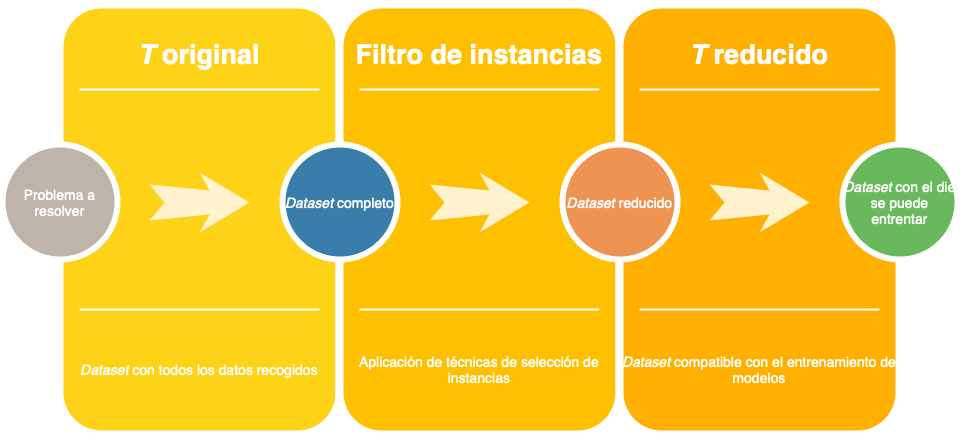
\includegraphics[width=\linewidth]{../img/memoria/Instance-Selection-Overview}
\caption{Proceso de selección de instancias.}
\label{fig:instance-election-overview}
\end{figure}

Es por ello que un pre-procesado o \textbf{filtrado} de las instancias pertenecientes al $T$ original es necesario. En la Figura~\ref{fig:instance-election-overview} se ilustra de manera gráfica el proceso de selección de instancias. Dado un conjunto de datos de entrenamiento inicial, $T$, el objetivo será obtener un subconjunto $S$, tal que $S \subseteq T$ de manera que $S$ no contiene instancias redundantes ni <<ruidosas>>. Además, $Acc(S) \cong Acc(T)$, donde $Acc(X)$ es la precisión, \textit{accuracy} en inglés, del modelo entrenado con el conjunto de datos $X$.

En función de cómo comienzan a crear el nuevo subconjunto de datos, $S$, se identifican dos aproximaciones, ascendente y descendente.
\begin{itemize}
\item \textbf{Ascendente.} El nuevo conjunto de datos comienza estando vacío, $S = \emptyset$, y a medida que se vayan realizando iteraciones del algoritmo correspondiente, se irán añadiendo instancias a $S$. El principal problema que posee esta aproximación es su sensibilidad al orden, \textit{i.e.} dada una instancia $x \subset T$, en diferentes iteraciones del mismo algoritmo de selección de instancias sobre el mismo $T$, puede o no estar en $S$. Esto se debe a la aleatoriedad con la que se presentan los datos, para asegurar esta aleatoriedad los datos se escogen de manera aleatoria de $T$, intrínsecamente da una mayor facilidad a las muestras iniciales a estar en $S$ que las finales, ya que puede que ya se encuentren representadas o sean clasificadas como ruido.

Entre las principales ventajas de esta aproximación destaca el espacio de almacenamiento requerido, puesto que se van guardando instancias y por lo tanto en un inicio es muy pequeño.

\item \textbf{Descendente.} El nuevo conjunto de datos comienza siendo el conjunto de entrenamiento al completo, $S = T$, y a medida que se vayan realizando las iteraciones del algoritmo correspondiente, se irán eliminando instancias de $S$. Esta aproximación es mucho más costosa computacionalmente, para cada instancia que debe decidir si eliminar o no debe comprobar todo el subconjunto $S$, pero en contraposición consigue reducir más que la aproximación ascendente, el conjunto de entrenamiento $T$.
\end{itemize}

Junto con esta diferenciación, en función de la aproximación de selección de instancias se pueden distinguir dos agrupaciones.
\begin{itemize}
\item \textbf{\textit{Wrapper}.} El criterio de selección se basa en la precisión del clasificador. Aquellas instancias que no contribuyen a la mejora del clasificador se quedan fuera de $S$. Este trabajo está centrado en este criterio de selección.
\item \textbf{\textit{Filter}.} El criterio de selección utiliza una función, $f(x, y)$, para realizar la selección, no se basa en un clasificador concreto.
\end{itemize}

\begin{table}[]
\small
\begin{center}
	\begin{tabular}{lcc}
	\toprule 
	\textbf{Método}  &  \textbf{\begin{tabular}[]{@{}c@{}}Complejidad\\Computacional\end{tabular}}  & \textbf{Referencia} \\
	\toprule
	\rowcolor[HTML]{EFEFEF} 
	Edición de Wilson (ENN)        & $O(n^2)$      &~\cite{wilson1972asymptotic}\\ 
	Condensado de Hart (CNN)     & $O(n^3)$         &~\cite{hart1968condensed}\\ 
	\rowcolor[HTML]{EFEFEF} 
	Condensado Reducido (RNN)     & $O(n^3)$         &~\cite{gates1972reduced}  \\ 
	\textit{Iterative Case Filtering} (ICF)     & $O(n^2)$              &~\cite{brighton2002advances}\\ 
	\rowcolor[HTML]{EFEFEF} 
	Subconjunto Selectivo Modificado (MSS)    & $O(n^2)$             &~\cite{barandela2005decision}\\ 
	\textit{Drecremental Reduction Optimization Procedure} (DROP) & $O(n^2)$  &~\cite{wilson2000reduction} \\ \bottomrule
	\end{tabular}
\end{center}
\caption{Algunos métodos de selección de instancias.}
\label{tab:instance-selection-methods}
\end{table}

En la Tabla~\ref{tab:instance-selection-methods} se aprecian aquellos algoritmos implementados en primera instancia para la reducción de instancias dentro de $T$, el objetivo de todos ellos es que el subconjunto generado, $S$, sea capaz de clasificar correctamente  $T$ en su totalidad prácticamente.

\subsubsection{Algoritmos de selección de instancias}\label{subsubsec:Instance-Selection-Algorithms}
Existen multitud de algoritmos a día de hoy que son capaces de reducir el número de instancias de $T$, en este trabajo se van a comentar los pertenecientes a la Tabla~\ref{tab:instance-selection-methods}. Cada uno de ellos tiene sus ventajas y sus desventajas como cabe esperar, en la literatura no apreciamos un <<este es mejor que aquel>> o similar.

\paragraph{Algoritmo de edición de Wilson}\label{paragraph:ENN}
\hfill \break
Wilson~\cite{wilson1972asymptotic} (1972) publicó la regla del vecino más cercano editado, \textit{ENN}. Los problemas de clasificación de instancias en función de una etiqueta, se caracterizan por:
\begin{itemize}
\item Hay una instancia a ser clasificada.
\item Existe un $S$ el cual posee instancias con la misma distribución que la instancia a clasificar, pudiendo ser comparables las instancias del conjunto con la que estamos analizando.
\item No existe información adicional del conjunto.
\item Existe una distancia medible entre instancias.
\end{itemize}

\begin{algorithm}[H]
	\KwIn{Conjunto de entrenamiento $X = \lbrace\left( x_1, y_1 ,\right)\dots \left(x_n, y_n\right)\rbrace$, $k$ número de vecinos.}
	\KwOut{Conjunto editado $S \subset X$}
  	\BlankLine
  	$S \leftarrow X$\\
  	\ForAll{$x \in S$}{
		Encontrar x.$N_{1\dots k+1}$, los $k$ + 1 vecinos más cercanos de $x \in X - \lbrace x \rbrace$\\
		\If{$\delta_{k-NN}\left(x_i\right)\neq \theta_i$}{
			Eliminar $x$ de $S$		
		}
  	}
  	\Return{$S$}
  \caption{Algoritmo de edición de Wilson, \textit{ENN}}\label{alg:Wilson-ENN}
\end{algorithm}

Con todas estas premisas Wilson propone un algoritmo basado en clasificación incorrecta en función de sus vecinos más cercanos. Cuando una instancia resulta mal clasificada por sus \textit{k} vecinos más cercanos, \textit{k}-NN, esa instancia es descartada. Finalmente obtendremos como resultado un conjunto $S$ con las instancias correctamente clasificadas por sus vecinos.

Suponiendo que sea \textit{X} un conjunto de \textit{N} instancias y \textit{M} posibles clases y, sea \textit{k} el número de vecinos cercanos, el algoritmo de Wilson se puede formular de la siguiente manera:

El algoritmo de edición de Wilson, ver algoritmo~\ref{alg:Wilson-ENN}, posee una complejidad computacional de $O(n^2)$. Una de las ventajas de este algoritmo es su forma de crear el subconjunto $S$, ya que al ser descendente las primeras iteraciones serán lentas --- dependiendo del tamaño de $T$ lógicamente --- pero las finales serán considerablemente más rápidas (siempre y cuando haya un nivel significativo de ruido).


\paragraph{Algoritmo Condensado de Hart}\label{paragraph:CNN}
\hfill \break
Hart~\cite{hart1968condensed} en 1968 propuso la que se considera la primera regla formal de condensador para NN. El algoritmo de condensado de Hart, \textit{CNN --- Condensed Nearest Neighbor}. Está basado en técnicas de consistencia y reducción. Sea $X \not= \emptyset$ y $S \subseteq X$, podremos decir que el subconjunto $S$ es consistente respecto al conjunto $X$ si al utilizar a $S$ como conjunto de aprendizaje, se puede clasificar correctamente a todo el conjunto $X$.

El algoritmo de Hart es una técnica ascendente, a partir de las primeras instancias que se añadan a $S$ se clasificarán y añadirán, o no, a $S$. Consiste en encontrar entre todas las instancias de $T$ un subconjunto $S$ tal que cada instancia de $T$ sea más cercano a las instancias en $S$ de su misma clase que a las instancias de otras clases, permitiendo utilizar $S$ como conjunto de clasificación de $T$. Para el correcto funcionamiento se asume que el conjunto $T$ es consistente, no posee dos instancias idénticas con pertenencia a diferentes clases.

El algoritmo propuesto por Hart~\cite{hart1968condensed}, ver algoritmo~\ref{alg:Hart-CNN}, posee una complejidad computacional de $O(n^2)$. El conjunto obtenido a partir de $T$, \textit{i.e.} $S$, operando con grandes conjuntos de datos demuestra poseer un tamaño considerablemente menor respecto a $T$. 

Si bien es una técnica utilizada por su efectividad, posee una serie de puntos negativos a su vez.
\begin{itemize}
\item Sensibilidad ante el ruido. Un objeto ruidoso no será correctamente clasificado por sus vecinos. Estas muestran no se eliminarán del conjunto solución $S$, por lo que no desaparecerán.
\item $S$ no tiene porqué ser el menor conjunto de $T$. Diferentes ejecuciones del algoritmo sobre el mismo $T$ pueden dar diferentes conjuntos solución $S$. Esto se debe al orden aleatorio por el cual se seleccionan las instancias. Por definición del propio algoritmo se asume que no se va a alcanzar de forma general el subconjunto de tamaño mínimo que cumpla con las características especificadas.
\end{itemize}

\begin{algorithm}[H]
	\KwIn{Conjunto de entrenamiento $X$}
	\KwOut{Conjunto editado $S \subset X$}
  	\BlankLine
  $S \leftarrow \left\lbrace x_1 \right\rbrace$\\
  	\ForAll{$x \in S$}{
		\If {$x$ no se clasifica correctamente usando $S$}{
			Añadir $x$ a $S$\\
			Reiniciar
		}
  	}
  	\Return{$S$}
	\caption{Algoritmo Condensado de Hart, \textit{CNN}.}\label{alg:Hart-CNN}
\end{algorithm}

\paragraph{Algoritmo Condensado Reducido}\label{paragraph:RNN}
\hfill \break
Gates~\cite{gates1972reduced} en 1972 propuso el algoritmo del conjunto reducido, basado en las reglas \textit{NN}. El algoritmo propuesto es una modificación del algoritmo \textit{CNN}, ver algoritmo~\ref{alg:Hart-CNN}. No es una nueva regla de decisión puesto que se sigue eligiendo la clase del vecino más cercano para la clasificación. 
El algoritmo se basa en un procedimiento para seleccionar el subconjunto $T_{CNN}$, el cual debe comportarse igual de bien que $T_{NN}$ ante clasificaciones de instancias desconocidas. Como se puede apreciar en el propio algoritmo~\ref{alg:Gates-RNN}, puede existir una disminución del rendimiento, a cambio se obtiene una mejora de la eficiencia para el algoritmo de clasificación que posteriormente se utilice, tanto en la cantidad de memoria utilizada como en el tiempo de computación.

De igual manera que en \textit{CNN}, posee la problemática de la minimalidad, si bien el conjunto resultante $S \subset T$ será consistente, no se puede asegurar que sea mínimo; y diferentes ejecuciones del algoritmo sobre el mismo conjunto de datos $T$, pueden obtener diferentes subconjuntos solución~$S$.

\begin{algorithm}[H]
	\KwIn{Conjunto de entrenamiento $X$}
	\KwOut{Conjunto editado $S \subset X$}
  	\BlankLine
  $S \leftarrow \left\lbrace x_1 \right\rbrace$\\
  	\ForAll{$x \in S$}{
		\If {$x$ no se clasifica correctamente usando $S$}{
			Añadir $x$ a $S$\\
			Reiniciar
		}
  	}
  	\ForAll {$x \in S$}{
			Eliminar $x$ de $S$\\
		\If {$\exists x_i$ incorrectamente clasificada usando $S$}{
			Añadir $x$ a $S$
		}
	}
  	\Return{$S$}
	\caption{Algoritmo Condensado Reducido, \textit{RNN}.}\label{alg:Gates-RNN}
\end{algorithm}

\paragraph{Algoritmo \textit{Iterative Case Filtering}}\label{subsubsub:ICF}
\hfill \break
Brighton~\cite{brighton2002advances} en 2002 propuso el algoritmo iterativo de filtrado, \textit{ICF}, bajo la premisa de predecir la clase de una instancia con la misma precisión, o mayor si fuera el caso, que el $T$ original. Uno de los objetivos principales del propio algoritmo es mantener en el subconjunto $S$ únicamente aquellas instancias que sean críticas para la decisión.

\textit{ICF} utiliza una estrategia decremental, \textit{i.e.} de manera iterativa va borrando instancias del conjunto de datos inicial, inicialmente realiza un filtrado y posteriormente la reducción~\cite{brighton2002advances} Al reducir el tamaño de $T$ los tiempos de respuesta para el proceso de clasificación mejorarán, ya que se examinarán un menor número de instancias para realizar la clasificación; por contrapartida al eliminar muestras que se creen que son dañinas para el proceso, se pueden estar eliminando algunas que sean clave y por lo tanto teniendo una degradación de la calidad del clasificador.

\textit{ICF} se basa en dos categorías para la decisión de si una instancia debe permanecer o no en $S$, ver algoritmo~\ref{alg:Brighton-ICF}, estas son \textit{Coverage} y \textit{Reachable}. Definidas de la siguiente manera para el caso base $\mathcal{CB} = \lbrace x_1, x_2, ..., x_n\rbrace$.
\begin{align*}
Coverage (x) = \lbrace x' \in \mathcal{CB} : Adaptable(x, x')\rbrace  \\
Reachable (x) = \lbrace x' \in \mathcal{CB} : Adaptable(x',x)\rbrace
\end{align*}

Una instancia $x$ podrá estar en el conjunto adaptable de $x'$ sí y solo si $x$ es una instancia relevante para la solución de $x'$, \textit{i.e.} $x \in k-NN(x)$. La problemática surge en el momento en el cual una instancia con clase diferente no permite la correcta clasificación de $x'$, es por ello que el vecindario de $x'$ viene definido por todas las instancias antes de la primera instancia de diferente clase, utilizando \textit{sets} descritos por Wilson y Martinez. La propiedad \textit{Reachable} no está fijada desde el principio del algoritmo, sino que es dinámica siendo fijada cada vez en función de la instancia de clase diferente más cercana. El criterio seguido para realizar la eliminación de una muestras es: si el \textit{set} formado por el $reachable(x)$ es mayor que el $coverage(x)$, \textit{i.e.} una instancia $x$ es eliminada cuando más instancias pueden resolver $x$ que las que $x$ puede resolver por sí misma.

\begin{algorithm}[H]
	\KwIn{Conjunto de entrenamiento $X$}
	\KwOut{Conjunto editado $T \subset X$}
  	\BlankLine
  \tcc{Filtro de ruido en función de la regla \textit{k-NN}}
  $T \leftarrow ENN(X,k)$\\  	
  \Repeat{no $progress$}{
  		\ForAll {$x \in T$}{  
  			Calcular $coverage(x)$\\
  			Calcular $reachable(x)$
  		}
  		$progress \leftarrow$ \textbf{false}\\
  		\ForAll {$x \in T$}{
			\If {$\left| reachable(x) \right| > \left| coverage(x) \right|$}{
				Marcar $x$ para eliminar\\
				$progress \leftarrow $ \textbf{true}
			}
		}
		\ForAll {$x \in T$}{
			\If{$x$ marcada para eliminar}{
				Eliminar $x$ de $T$
			}
		}
  }
  	\Return{$T$}
	\caption{\textit{Iterative Case Filtering}, \textit{ICF}.}\label{alg:Brighton-ICF}
\end{algorithm}

\paragraph{Algoritmo Subconjunto Selectivo}\label{paragraph:SS}
\hfill \break
Ritter~\cite{ritter1975algorithm} 1975 propone un algoritmo capaz de satisfacer la condición de consistencia del algoritmo condensado de Hart, ver algoritmo~\ref{alg:Hart-CNN}; para ello introduce una condición más <<fuerte>> de consistencia, el objetivo es encontrar aquellas instancias de un orden independiente. 

Un subconjunto $S$ del conjunto de entrenamiento $T$, es un Subconjunto Selectivo, $SS$, si $SS$ cumple las siguientes condiciones:
\begin{enumerate}
\item El subconjunto $S$ debe ser consistente.
\item Todas las instancias tiene que ser más cercanas a un vecino selectivo de la misma clase que a cualquier otra instancia de otra clase.
\item No puede haber ningún subconjunto $S'$ que satisfaga las condiciones 1 y 2, y que al mismo tiempo contenga un menor número de instancias que el Subconjunto Selectivo, $SS$.
\end{enumerate}

La segunda condición es la diferencia principal entre el algoritmo de Hart y el subconjunto calculado con el algoritmo del subconjunto selectivo. De forma que se puede re-formular el punto número dos de la siguiente manera:

\emph{Todas las instancias del conjunto de entrenamiento $T$ deben de ser más cercanos a un vecino condensado --- miembro del subconjunto condensado $\mathcal{CS}$ --- de la misma clase que a cualquier otra instancia de otra clase diferente del $\mathcal{CS}$.}

Pudiendo verse como una reformulación del punto nº 1. Además, el punto nº  2 para el subconjunto selectivo permite un subconjunto de menor tamaño, eliminando la necesidad de calcular todas las permutaciones de las instancias en $T$. Con unos criterios más específicos que los que se encuentran en el algoritmo condensado, el subconjunto selectivo resultante no tiene porqué ser mínimamente consistente. Asimismo, de forma general, no será un subconjunto reducido del $S$ producido por \textit{CNN}.


\paragraph{Algoritmo Subconjunto Selectivo Modificado}\label{paragraph:MSS}
\hfill \break
Barandela~\cite{barandela2005decision} 2005 propuso el algoritmo de subconjunto selectivo modificado, \textit{MSS}, como su propio nombre indica, se trata de una modificación del algoritmo Subconjunto Selectivo, SS. Debido a que no se puede garantizar que el algoritmo de Ritter~\cite{ritter1975algorithm} devuelva un subconjunto, $S$, el cual sea mínimo y consistente, habiendo sido categorizado como un problema NP-Completo~\cite{wilfong1992nearest}, por lo que \textit{MSS} pretende conseguir el subconjunto mínimo consistente mediante el uso de la propiedad selectiva.

La aproximación realizada por Barandela \textit{et al.} modifica la condición nº 3 anteriormente propuesta, mientras que las nº 1 y 2 no son modificadas. De forma que la definición nº 3 queda formulada de la siguiente manera:

\emph{El Subconjunto Selectivo Modificado, \textit{MSS}, se define como el subconjunto del conjunto de entrenamiento $TS$, el cual $\forall x_i \in TS$ aquella instancia de $Y_i$ qiue es más cercano a otra clase que a la de $x_i$, \textit{i.e.} el más cercano a su enemigo más cercano.}


El objetivo principal de esta modificación es reforzar la condición que debe cumplir el subconjunto reducido para maximizar la aproximación a la frontera de decisión. Quedando definido el algoritmo, ver algoritmo~\ref{alg:Barandela-MSS}, como una alternativa eficiente al algoritmo propuesto por Ritter \textit{et al.}, siendo capaz de seleccionar mejores instancias (más cercanas a la frontera de decisión). 

El criterio que sigue \textit{MSS} para determinar la frontera de decisión es la distancia al enemigo más cercano. Con esta medida se puede definir el mejor subconjunto selectivo como aquel que contiene el mejor vecino relacionado para cada instancia en el $TS$. (Mejor $\iff$ Menor distancia a su enemigo más cercano).

\begin{algorithm}[H]
	\KwIn{Conjunto de entrenamiento $X$}
	\KwOut{Conjunto editado $S \subset X$}
  	\BlankLine
  $S \leftarrow \emptyset$\\  	
  Ordenar las instancias $\lbrace x_i \rbrace^{n}_{i=1}$ en función de $D_i$ a su enemigo más cercano\\
  \For {$i = 1$ hasta $n$}{
		$add \leftarrow$ \textbf{false}\\
		\For {$j=i$ hasta $n$}{
			\If {$x_j \in T \bigwedge d\left( x_i, x_j \right) < D_j$}{
				 Eliminar $x_j$ de $T$\\
				 $add \leftarrow$ \textbf{true}
			}
		}
		\If {$add$}{
			Añadir $x_i$ a $S$
		} 
		\If {$T = \emptyset$}{
			\textbf{return} $S$
		}
	}
	\caption{\textit{Modified Selective Subset}, \textit{MSS}.}\label{alg:Barandela-MSS}
\end{algorithm}

\paragraph{\textit{Decremental Reduction Optimization Procedure}}\label{paragraph:DROP}
\hfill \break
Bajo el nombre de \textit{Decremental Reduction Optimization Procedure, DROP}~\cite{wilson2000reduction} nos encontramos con hasta 5 aproximaciones para la resolución del mismo problema. Todas ellas seleccionan prototipos en función de \textit{socio} y \textit{asociado}. Definidos como:
\begin{itemize}
\item Socio. Sea $X \not= \emptyset$, el socio de un objeto $P$ el cual pertenece al conjunto $X$, es aquél objeto que tiene a $P$ como uno de sus $k$ vecinos más cercanos.
\item Asociado. Todo prototipo que contenga a $P$ como a uno de sus $k$ vecinos más cercanos, será denominado asociado de $P$, denotado con la expresión $P.A_{1,\dots,a}$ donde $a$ es el número de asociados de $P$.
\end{itemize}

Volviendo sobre los conceptos de \textit{coverage} y \textit{reachable} vistos en el algoritmo \textit{Iterative Case Filtering}, (ICF), podemos relacionar todos los conceptos de la siguiente manera: los asociados de un prototipo $P$ se pueden ver como el conjunto formado por el \textit{reachable} de $P$, y con el \textit{coverage} se pueden obtener los socios del prototipo $P$.

Todas las aproximaciones de $DROP\lbrace 1\dots5\rbrace$ se basan en el mismo algoritmo~\cite{wilson2000reduction} pero con modificaciones en las técnicas de pre-procesado de los prototipos. Sus diferencias son:
\begin{itemize}
\item \textit{DROP1}. Eliminará un objeto $P$ de $S$ si sus socios en $S$ se clasifican correctamente sin $P$, \textit{i.e.} la ausencia de $P$ no impide la correcta clasificación del resto de prototipos.
\item \textit{DROP2}. Eliminará un objeto $P$ de $S$ si los socios que tiene $P$ en $TS$ se clasifican correctamente sin $P$, \textit{i.e.}, verificará el efecto que causa esta eliminación sobre la muestra original. Previo al proceso de eliminación de objetos $P$, ordena los prototipos a tratar en orden a su enemigo más cercano, permitiendo que los primeros prototipos que se van a tratar serán aquellos más alejados de las fronteras de decisión, ergo las más prescindibles.
\item \textit{DROP3}. Lo primero de todo realiza un filtrado de ruido, para ello aplica la edición de Wilson, ver algoritmo~\ref{alg:Wilson-ENN}. Seguidamente aplica el algoritmo \textit{DROP2}, ver algoritmo~\ref{alg:DROP3}
\item \textit{DROP4}. Aplica un filtro de ruido diferente, en este casos consistirá en eliminar un prototipo solo si su eliminación no provoca que alguna otra instancia sea mal clasificada.
\item \textit{DROP5}. Modificación sobre \textit{DROP2}, en este algoritmo el proceso de eliminación de objetos comienza por aquellos más cercanos a sus enemigos. 
\end{itemize}

El concepto \textit{with} permite recoger el número de asociados correctamente clasificados teniendo en cuenta un prototipo $x$ como vecino, en cambio \textit{without} tiene en cuenta el número de asociados correctamente clasificados los cuales no tienen el prototipo $x$ como vecino. En los casos en los que $without > with$ se está tratando con un prototipo el cual no aporta información sobre el conjunto $S$ permitiendo su eliminación.

\begin{algorithm}[H]
	\KwIn{Conjunto de entrenamiento $X$ y número de vecinos más cercanos a considerar, $k$}
	\KwOut{Conjunto editado $S \subset X$}
  	\BlankLine
  $S \leftarrow \text{Filtrado de ruido}(X)$ \\
	Ordenar las instancias de $S$ por la distancia a su enemigo más próximo \tcc*[f]{de mayor a menor}\\
	\ForAll{$x \in S$}{
		Encontrar los $x.N_{1\dots k+1}$, los $k+1$ vecinos más cercanos de $x$ en $S$\\
		Añadir $x$ a la lista de asociados de cada uno de sus vecinos
	}
	\ForAll{$x \in S$}{
		$with \leftarrow$ número de asociados de $x$ clasificados correctamente \textbf{con} $x$ como vecino\\
		$without \leftarrow$ número de asociados de $x$ clasificados correctamente \textbf{sin} $x$ como vecino\\
		\If{$without \geq with$}{
			Eliminar $x$ de $S$\\
			\ForAll{Asociado $a$ de $x$}{
				Eliminar $x$ de la lista de vecinos de $a$\\
				Encontrar nuevo vecino para $a$\\
				Añadir $a$ en la lista de asociados del nuevo vecino
			}
		}
	}
	\Return{$S$}
	\caption{\textit{Decremental Reduction Optimization Procedure 3}, \textit{DROP3}.}\label{alg:DROP3}
\end{algorithm}

\section{Función distancia entre instancias}
Una función distancia proporciona información sobre la proximidad entre dos instancias en función de todos sus parámetros. Si la distancia que separa dos instancias es cero, ambas instancias son idénticas. Se tiende a trabajar con conjuntos de datos normalizados, \textit{i.e.} todos los datos son ajustados a una escala común, independientemente de la escala en la que hayan sido medidos, para evitar que atributos/características con mucha varianza puedan <<despistar>> a los algoritmos.

Existen multitud de métricas para calcular la distancia, pudiendo variar la distancia calculada en función de cuál se aplique. Se van a comentar las más representativas.
\begin{itemize}
\item \textbf{Distancia de Minkowski.} La distancia de Minkowski es una métrica en el espacio vectorial normalizado. Es una métrica que se puede modificar con facilidad para calcular la distancia entre dos instancias de diferentes maneras. 
\begin{enumerate}
\item \(p = 1\), cálculo de la distancia de Manhattan.
\item \(p = 2\), cálculo de la distancia Euclídea.
\item \(p = \infty\), cálculo de la distancia de Chebyshov.
\end{enumerate}
Su fórmula es la siguiente:
\[ \mathbb{D}(x, y) = \left( \sum_{i=1}^{n}\left| x_i - y_i \right|^p \right)^{1/p} \]

\item \textbf{Distancia de Manhattan} o distancia del taxista. Es una métrica en un espacio vectorial normalizado, calculándose como la suma de los $n$ segmentos verticales u horizontales que unen dos puntos.

Su fórmula es la siguiente:
\[  \mathbb{D}(x, y) = \sum_{i=1}^{d}\left| x_i - y_i\right| \]

\item \textbf{Distancia euclidiana} o norma L2 o distancia L2. Es la distancia en línea recta entre dos puntos de datos en el espacio euclidiano.

Su fórmula normalizada es la siguiente:
\[  \mathbb{D}(x, y) = \sqrt{\sum_{i=1}^{d} \frac{\left(x_i - y_i\right)^2}{\sigma_i^2}}  \]

\item \textbf{Distancia de Chebyshov} o distancia del tablero de ajedrez. La distancia entre dos puntos es la mayor de sus diferencias a lo largo de cualquiera de sus dimensiones coordenadas.

Su fórmula es la siguiente:
\[  \mathbb{D}(x, y) = \max_i\left(\left|x_i - y_i\right|\right) \]

\end{itemize}
